%% The following is a directive for TeXShop to indicate the main file
%!TEX root = ../MJThesis.tex
%\bibliography{../misc/bibli}
\acresetall{}

\chapter{Introduction}
\label{ch:Introduction}

\begin{epigraph} \emph{``But during the writing of this review, I learned how little I knew in this
    area, and this was a humbling and sobering experience. I am certain that I have made many
    mistakes due to my ignorance, and I hope that the review will be useful despite its many faults''}\\
  ---~Hiroshi Nikaido, 2003, my grand supervisor.
\end{epigraph}
\section{S-layers} \label{sec:intro-slayers}
\subsection{S-layer structure} % (fold)
\label{sub:s_layer_structure} \lettrine[lines=2]{C}{ellular} envelopes are the interface between a
cell and its environment. Many different organsims have evolved extra coatings and membrane
adaptations to enhance or provide new functionality to their cell envelopes. For example, capsules
can enhance the virulence of \textit{Streptococci}\upcite[]{griffith1928significance} and mycolic
acids increase resistance to antibiotics for \textit{Mycobacteria}\upcite[.]{nguyen2006foundations}
One such adaptation widespread in microbially life is the \ac{S-layer}. \Acp{S-layer} are
proteinacious, para-crystalline coatings that surround some bacteria and
archaea\upcite[.]{beveridge1991surface, sara2000s}. A good review on the subject of \ac{S-layer} structure was written by Tea Pavkov-Keller, Stefan Howorka and Walter Keller\upcite[.]{PavkovKeller201173} \Acp{S-layer} are planar, being a thin layer of protein or glycoprotein sitting externally to outer membrane in Gram-negative bacteria, the
peptidoglycan layer in Gram-positive bacteria, and the cell membrane of
archaeabacteria. \Cref{fig:cellwalls} (\vpageref{fig:cellwalls}) diagrams the general,
cross-sectional structure of bacteria and archaea that possess an S-layer.

\begin{figure}[htb] % Cell  envelopes diagrams
  \begin{center}
    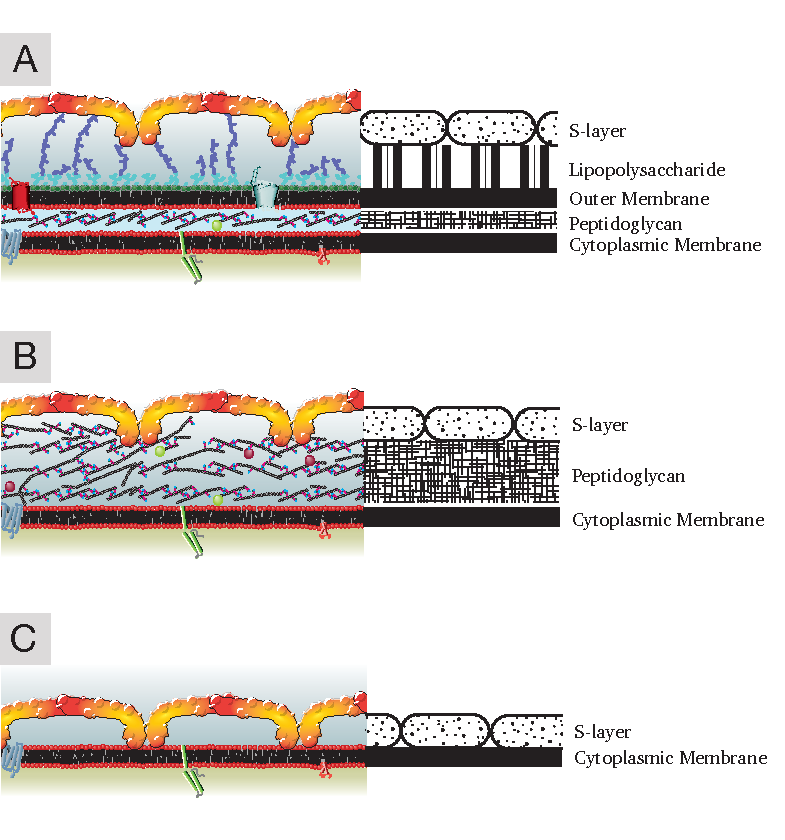
\includegraphics{intro/img/celwalls.pdf}
  \end{center}
  \caption[Cross-sectional diagrams of \ac{S-layer} containing cell envelopes]{Cross-sectional
    diagrams of the cell envelopes of (\textbf{A}) Gram negative bacteria, (\textbf{B}) Gram
    positive bacteria, and (\textbf{C}) archaebacteria. In all known cases the \ac{S-layer} sits on
    the extreme outer surface of the cell. (This diagram was inspired by Fig. 1 from
    \fullcite{sleytr1983crystalline})}
  \label{fig:cellwalls}
\end{figure}

\Acp{S-layer} are composed of one or only a few proteins or glycoproteins. In most known examples,
\acp{S-layer} are composed of just one repeated protein, in a few cases \acp{S-layer} are composed
of a few separate proteins. The \ac{S-layer} from \textit{Clostridium difficile} is composed of two
proteins (HMW and LMW) that arise from the cleavage of a single precursor protein (SlpA) that is
cleaved during secretion\upcite[.]{calabi2001difficile, fagan2009difficile} \textit{Bacillus
  anthracis} has a \ac{S-layer} that is composed of two proteins (EA1 and Sap) that are individually
expressed and assemble together on the surface of the bacterium\upcite[.]{mesnage1997molecular}
Interestingly, \textit{Brevibacillus brevis} appears to have two \acp{S-layer} stacked on top of each
other; the outer layer having oblique symmetry and the lower layer having hexagonal
symmetry\upcite[.]{sara1990brevis}
    
For \acp{S-layer} that are composed of a single protein, that protein is repeated thousands of times
across the surface of the cell and is arranged in a regular geometric pattern. The geometric
patterns can be observed by electron microscopy. The traditional electron microscopy techniques of freeze fracture and negative stain have been the most successful techniques historically to see \acp{S-layer} and \ac{S-layer} geometries\upcite[.]{smit1981periodic} The six major geometric symmetries found in
\acp{S-layer} are oblique (p1 and p2), triangular (p3), rectangular (p4), and hexagonal
(p6). \Cref{fig:symmetries} (\vpageref{fig:symmetries}) features simple examples of the six major
symmetries found in \acp{S-layer}.  Examples of bacteria with oblique \acp{S-layer} are
\textit{Bacillus stearothermophilus} NRS2004$/$3a\upcite{messner1986characterization} and
\textit{Brevibacillus brevis}\upcite[.]{masuda1980reassembly} Examples of bacteria with rectangular
\acp{S-layer} are \textit{Corynebacterium
  diptheriae}e\upcite{kawata1972extracellular} and \ac{aeromonas}
A450\upcite[.]{ishiguro1981loss} An example of a bacterium with a
triangular \ac{S-layer} is \textit{Sulfolobus acidocaldarius}\upcite[.]{weiss1974subunit} Examples
of bacteria with hexagonal \acp{S-layer} are \textit{Bacillus anthracis}\upcite{holt1969comparative}
and \textit{Caulobacter crescentus} CB15\upcite[.]{smit1981periodic}

\begin{figure}[htb] % S-layer symmetries
  \begin{center}
    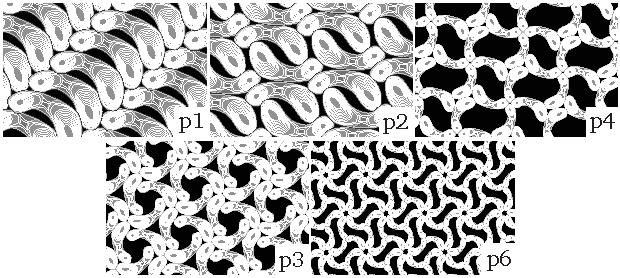
\includegraphics[]{intro/img/symmetries.pdf}
  \end{center}
  \caption[A simple overview of \ac{S-layer} symmetries]{A simple overview of \ac{S-layer}
    symmetries. p1 and p2 are oblique symmetries.  p4 is a rectangular symmetry.  p3 is a triangular
    symmetry.  p6 is a hexagonal symmetry.}
  \label{fig:symmetries}
\end{figure}
   
In addition to the traditional transmission electron microscopy techniques that have been used to
visualize bacterial cell surfaces in the past, a new method of cryo-electron tomography has been
used recently to observe and dissect bacterial cells. Cryo-electron tomography has the advantage
that it be used to observe unfixed and unstained intact cells. Being a tomographical technique cross
sections can be reconstructed to observe the fine structure within and on a bacterial cell. No
deliberate study has been taken to use cryo-electron tomography to study \acp{S-layer}, but their
presence is easily observed in the fantastic images produced by other studies utilizing the
technique. This technique has been pioneered for use in bacteria and specifically in \ac{caulobacter} by the laboratory of Dr.\,Grant Jensen at the California Institute of Technology. \Cref{fig:intro-tomo} (\vpageref{fig:intro-tomo}) features a tomographical cross-section of a \ac{caulobacter} cell; visible is the inner and outer membranes and the \ac{S-layer} composed of the protein RsaA.

\begin{figure}[htb]
  \begin{center}
    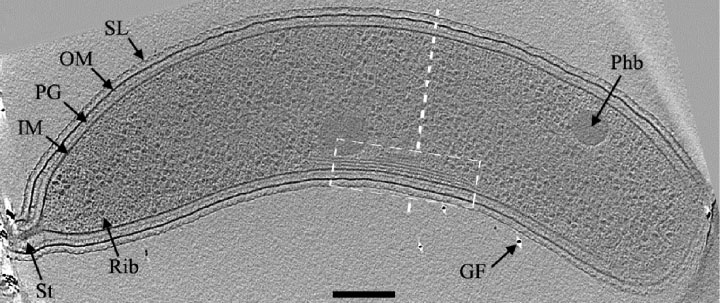
\includegraphics[width=0.8\textwidth]{intro/img/jensentomograph.jpg}
  \end{center}
  \caption[Electrotomograph of \ac{caulobacter}]{ The location of the \ac{S-layer} is around the
    exterior of the cell, as can be seen in this image. The figure is a 19 \si{\nano\meter}
    cross-section through the three-dimensional reconstruction of one representative
    \ac{caulobacter} cell, perpendicular to the direction of the beam: \textbf{SL}, surface layer;
    \textbf{OM}, outer membrane; \textbf{PG}, peptidoglycan layer; \textbf{IM}, inner membrane;
    \textbf{St}, stalk; \textbf{Rib}, probable ribosome; \textbf{GF}, gold fiducial used to align
    images; \textbf{Phb}, putative poly-$\beta$-hydroxybutyrate granule. The scale bar indicates 200 \si{\nano\meter}. (This figure is a portion of Figure 1 from \fullcite{Jensen2006tomo}. Reused
    with full permission from the publisher, Wiley.)}
  \label{fig:intro-tomo}
\end{figure}

\subsection{S-layer Proteins} \label{sub:intro-slayerproteins} % S-layer protein subsection

Discussing \ac{S-layer} proteins on a whole can be difficult because \ac{S-layer} proteins don't represent a monophyletic group of related molecules; \ac{S-layer} proteins seem to be distinctly unrelated proteins that share a common cellular location and gross structure through convergent evolution. One of the best reviews on \ac{S-layer} proteins was published in 2000 by Margit S\'{a}ra and Uwe B. Sleytr\upcite[.]{sara2000s} 

\ac{S-layer} proteins do tend to share similar properties and overall composition. \ac{S-layer} proteins are large proteins. For the \ac{S-layer} proteins whose sequences are known, all are larger than 400 \acp{aa} and many of them larger than 1000 \acp{aa}\upcite[.]{sara2000s} The amino acids in \ac{S-layer} proteins are rich in hydrophobic and negatively charged residues, low in methionines, and  cysteines are almost completely unrepresented\upcite[.]{gilchrist1992nucleotide, sara2000s, vilen2009surface}  

\ac{S-layer} proteins are almost universally glycosylated in \textit{Archaeabacteria}, commonly
glycosylated in Gram-positive bacteria, and very rarely glycosylated in Gram-negative
bacteria\upcite[.]{sara2000s, lechner1989structure}
For some microbes, the \ac{S-layer}'s main function maybe as a platform for oligo/polysaccharide chains. One study by Sch\"{a}ffer et\,al.~asked the question about the glycosylation of \ac{S-layer} proteins, ``Are \ac{S-layer} Glycoproteins and Lipopolysaccharide Related?''\upcite[]{schaffer1996s} The study identified structural similarities between the carbohydrates in \ac{OPS} and the carbohydrates on glycosylated \ac{S-layer} proteins; pointing out they have more in common with each other than with eukaryotic polysaccharides. The study makes great leaps from sugar structures to phylogenetic and taxonomic conclusions, but the study does highlight that supporting a highly glycosylated surface is a widespread feature in microbially life and it is a role that \ac{S-layer} proteins serve in some organisms. Role of glycosylation and the functions served by \acp{S-layer} is further discussed in \cref{sec:intro-slayersfunction}.
% subsection s_layer_structure (end)

  \subsection{Functions of S-layers}
  \label{sec:intro-slayersfunction}

  As mentioned before, \acp{S-layer} are not a single family of realte proteins---likewise the do not fill the same needs in all species. Interestingly, despite the apparent convergent evolution in many disparate organisms pushing towards a widespread similarity in structure and composition, \acp{S-layer} seemingly perform many  different functions. Further, \acp{S-layer} require a large metabolic commitment to produce and despite that, they are still retained in many species where their functions are enigmatic.

  \paragraph{Pathogenic bacteria} For pathogenic bacteria, a \ac{S-layer} is often a virulence factor. In \ac{anthrax}, the \ac{S-layer} consists of the protein BslA and it functions as an adhesin\upcite[.]{kern2010bsla} BslA is sufficient and required for \ac{anthrax} to adhere to host cells and mutants that lack the \ac{S-layer} have much reduced virulence and increased time-to-death in animal models. Due to their location on the surface of the cell, \acp{S-layer} functioning as adhesins is a common theme in pathogens. \ac{aeromonas} has a \ac{S-layer} that also functions as an adhesin\upcite[.]{garduno2000host} The \ac{aeromonas} \ac{S-layer} binds to both fibronectin and laminin on host cell surfaces\upcite[]{doig1992binding} but is not involved or required for host cell invasion (probably mediated by the \ac{LPS})\upcite[.]{garduno2000host}
  The \ac{aeromonas} \ac{S-layer} is sufficient to confere host cell adhesion to the bacterial cells and also to nylon microbeads \textit{in vitro} that have been coated with the \ac{aeromonas} \ac{S-layer} protein, VapA. 

  For \ac{cfetus}, its \ac{S-layer} is central to its success as a pathogen of ungulates. The \ac{S-layer} of \ac{cfetus} is involved in disseminating the bacteria throughout the host's body and evading the host immune system\upcite[.]{thompson2002campylobacter} The manner is which \ac{cfetus} uses its \ac{S-layer} to escape the immune system is remarkable. The \ac{S-layer} provides the cells with an innate resistance to complement, strains with an intact \ac{S-layer} bound less C3 protein than cells lacking a \ac{S-layer}. By binding less C3, \ac{S-layer} positive \ac{cfetus} prevent complement-mediated killing and opsonization by C3b. The \ac{S-layer} would be a natural target for antibody-mediated adaptive immunity, but \ac{cfetus} has also evolved a strategy to escape antibody recognition. \ac{cfetus} possess the ability to undergo antigenic conversion by expressing different versions of its \ac{S-layer}. The \ac{cfetus} cells can invert portions of their genomic DNA to express alternate \ac{S-layer} proteins and cognate \ac{OPS} anchor molecules. As an example, the \ac{cfetus} serotype A strain 23D encodes for eight different \ac{S-layer} proteins and can switch between expressing each by moving a single active promoter in front of the \ac{S-layer} protein gene to be expressed. These \acp{S-layer} are not just different antigenically, they can even form different symmetry patterns (see \cref{fig:symmetries} on \vpageref{fig:symmetries}).

\paragraph{Non-pathogenic bacteria}  %% Intro paragraph
\acp{s-layer} acting as a physical barrier, protecting the cell, is a function primarily exemplified \caulobacter and other gram-negative bacteria possessing an \ac{s-layer}. Susan Koval of the university of western ontario has done extensive research into the biology and life-cycle of \textit{bdellovibrio} spp. and \textit{bdellovibrio}-like species, predatory bacteria that prey on gram-negative bacteria like \caulobacter. Koval showed that the \ac{S-layer} of \caulobacter had a protective effect against \textit{bdellovibrio} predation\upcite[.]{koval1991effect} This protective effect was seen for  \ac{aeromonas}, \textit{Aquaspirillum serpens}, \textit{Aquaspirillum sinuosum}, \ac{cfetus}, and \caulobacter. On the other hand, \acp{S-layer} do not confer any protection from predation by protozoans (\eg{} \textit{Tetrahymena thermophila} and \textit{Paraphysomonas vestita})\upcite[.]{koval1993predation}

Due to their location around the outside of a cell, \acp{S-layer} are in a prime position to modify the surface the chemical and physical characteristics of a microbe. It has been noted that many bacteria with an \ac{S-layer} are more hydrophobic than isogenic variants lacking an \ac{S-layer}\upcite[.]{beveridge1997v} A noted exception to the hydrophobicity observations was for \caulobacter strains CB2A and CB2NY66R, possibly its \ac{S-layer} covers beneath it a more hydrophobic outer membrane (see \cref{ch:lps} on \cpageref{ch:lps} for our research on the \caulobcter \ac{LPS}). Beyond changing the general chemical properties of the cell surface, \acp{S-layer} also change the cell surface to provide a specific site for extracellular proteins to anchor. Enzymes that are secreted, but remain associated with the cell, can use \acp{S-layer} as display platforms. The enzyme pullulanase in \textit{Clostridium thermosulfurogenes} anchors itself into the \ac{S-layer} with three C-terminal regions that have a significant sequence \ac{S-layer}\upcite[.]{matuschek1994pullulanase} It's thought that the \textit{C. thermosulfurogenes} pullulanase integrates itself in the lattice of the \ac{S-layer} in order to anchor itself. Intergration into the \ac{S-layer} is not the strategy used by \textit{Geobacillus stearothermophilus} DSM2358 and its amylases. The high molecular weight amylase from \textit{G. stearothermophilus} binds the cell surface but without any detectable interaction with peptidoglycan, instead it associates with \ac{S-layer} in a manner that is specifically not lattice integration\upcite[.]{egelseer1995s}


  \subsection{History of S-layers} % (fold)
  \label{sub:history_of_s_layers}

  \begin{figure}[htb] % First S-layer
    \begin{center}
      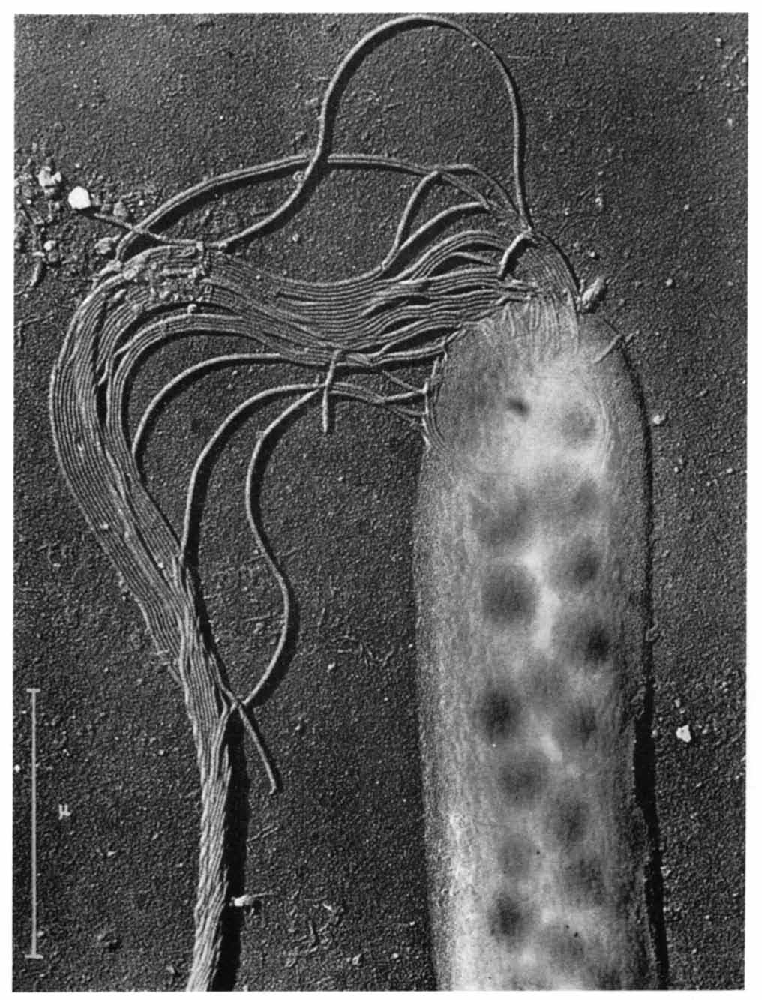
\includegraphics{intro/img/firstslayer.pdf}
    \end{center}
    \caption[The first published image of a \ac{S-layer}]{The first published image of a
      \ac{S-layer}. The hexagonal \ac{S-layer} on the surface of the bacterium --- probably
      \textit{Spirillum} sp. --- is visible along the edges of the cell body (centre right). The scale
      bar denotes one micrometre. (This image is Figure 1 from \fullcite{firstslayer}. Reused with
      full permission from the publisher, Elsevier.)}
    \label{fig:firstslayer}
  \end{figure} % section history_of_s_layers (end)
  % section paracrystalline_protein_surface_layers (end)

  \subsection{RsaA} \label{sec:intro-rsaa}

  RsaA, named for \underline{r}egular \underline{s}urface \underline{a}rray\upcite[,]{gilchrist1991transformation} is a 1026 \ac{aa} protein from \caulobacter with an average \ac{mw} of 98001.70 Da and an \ac{pi} of 3.85. The amino acid sequence of RsaA can be found in the appendix on \cpageref{app:rsaseq}. The \ac{S-layer} of \caulobacter comprises roughly 45000 copies\upcite[]{slayercryo} of RsaA arranged in an p6 symmetry (see \cref{fig:symmetries} on \cpageref{fig:symmetries}). \Cref{fig:intro-micrograph} displays a computer generated view of the surface of the \ac{S-layer} of \caulobacter as determined by electron microscopy. RsaA is a \ac{t1ss} secreted protein containing six \ac{rtx} motifs.

  \begin{figure}[htb]
    \begin{center}
      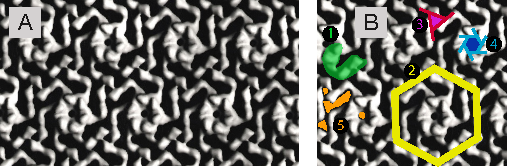
\includegraphics[width=\textwidth]{intro/img/slayermicrograph.pdf}
    \end{center}
    \caption[Reconstructed surface of the \caulobacter \ac{S-layer}]{
      The surface structure of the \ac{S-layer} from \caulobacter, reconstructed from tilt-series electron microscopy. \textbf{A.} An section of reconstructed surface of the \caulobacter \ac{S-layer}. The image shown is in a left-handed configuration, except the handedness of the \ac{S-layer} couldn't be determined in the original study, therefore this image may be a mirror image of the true configuration of the \ac{S-layer}. \textbf{B.} Interpretations of the micrograph.  A monomer of RsaA is highlighted in green (\textit{B.1}).  The unit cell of the \ac{S-layer} is six copies of RsaA arranged in a hexagonal pattern (\textit{B.2}).  The center of three-fold symmetry, red, is comprised of the N-termini of RsaA (\textit{B.3}).  The C-termini of the RsaA monomers face towards each other in the center of the point of six-fold symmetry, blue (\textit{B.4}). (This image is derived from Figure 6 from \fullcite{smit1992s})
    }
    \label{fig:intro-micrograph}
  \end{figure}   

  \paragraph{Type 1 secretion} RsaA is secreted by a \ac{t1ss}. \Ac{t1ss} secreted proteins are secreted in one step across both the inner and outer membranes of Gram-negative bacteria. A \ac{t1ss} requires three components: an inner membrane spanning \ac{abc} transporter, a periplasm spanning membrane fusion protein, and an outer membrane protein. For RsaA's secretion from \caulobacter, these proteins are RsaD, RsaE, and RsaF (either RsaFa or RsaFb). Like all \ac{t1ss} secreted proteins, RsaA is secreted starting from the C-terminus to the N-terminus. As proteins are translated from the N-terminus to the C-terminus, all \ac{t1ss} secreted proteins (including RsaA) exist in the cytoplasm as fully translated polypeptides prior to secretion. This is in contrast to protein secreted by N-terminus first means, which allow for the possibility for secretion to begin on a nascent peptide before translation is complete. The diameter of \ac{t1ss} pore is not wide enough to accommodate the secretion of a fully folded protein, so \ac{t1ss} secreted proteins often have a C-terminus that is intrinsically disordered prior to secretion; this disordered state is mediated by \ac{rtx} motifs\upcite[.]{chenal2009rtx}   

  % TODO add citations to above paragraph

  \paragraph{Repeat-in-toxin motifs} First identified in the \ecoli protein $\alpha$-haemolysin (HlyA)\upcite[,]{felmlee1988alterations} \ac{rtx} motifs are a nearly ubiquitous component of \ac{t1ss} secreted proteins. Despite the name, \acl{rtx} aren't exclusively found in toxins, they are found in many classes of protein, lipases, proteases, S-layers,\textit{etc.}  \ac{rtx} motifs are small peptide sequences, typically 6--9 \ac{aa} in length:\texttt{GGXGXD}\upcite[]{letoffe1992secretion} or \texttt{GGXGXDXLX}(where \texttt{G} is glycine, \texttt{D} is aspartate, \texttt{X} can be any amino acid, and \texttt{L} is leucine but is often substituted for valine, isoleucine, phenylalanine, or tyrosine)\upcite[.]{rose1995interaction, chenal2009rtx} The short sequences are always present in multiples (6--50+), often found in tandem repeats. Each \ac{rtx} motif forms two half sites for binding \ce{Ca^2+}, which can collaborate with other neighbouring \ac{rtx} sites to coordinate ions and stabilize a connection between disparate regions of a protein. Upon binding \ce{Ca^2+}, \ac{rtx} motifs assume a parallel $\beta$-roll fold\upcite[,]{meier2007calcium} rolling around \ce{Ca^2+} ions at the turns. An example of a \ac{rtx} $\beta$-roll structure can be found in \cref{fig:intro-rtx}.
  % The reported \ac{kd} of \ac{rtx} sites is 0.5--0.8 \millimolar\upcite[.]{rose1995interaction} 

  \begin{figure}[htb]
    \begin{center}
      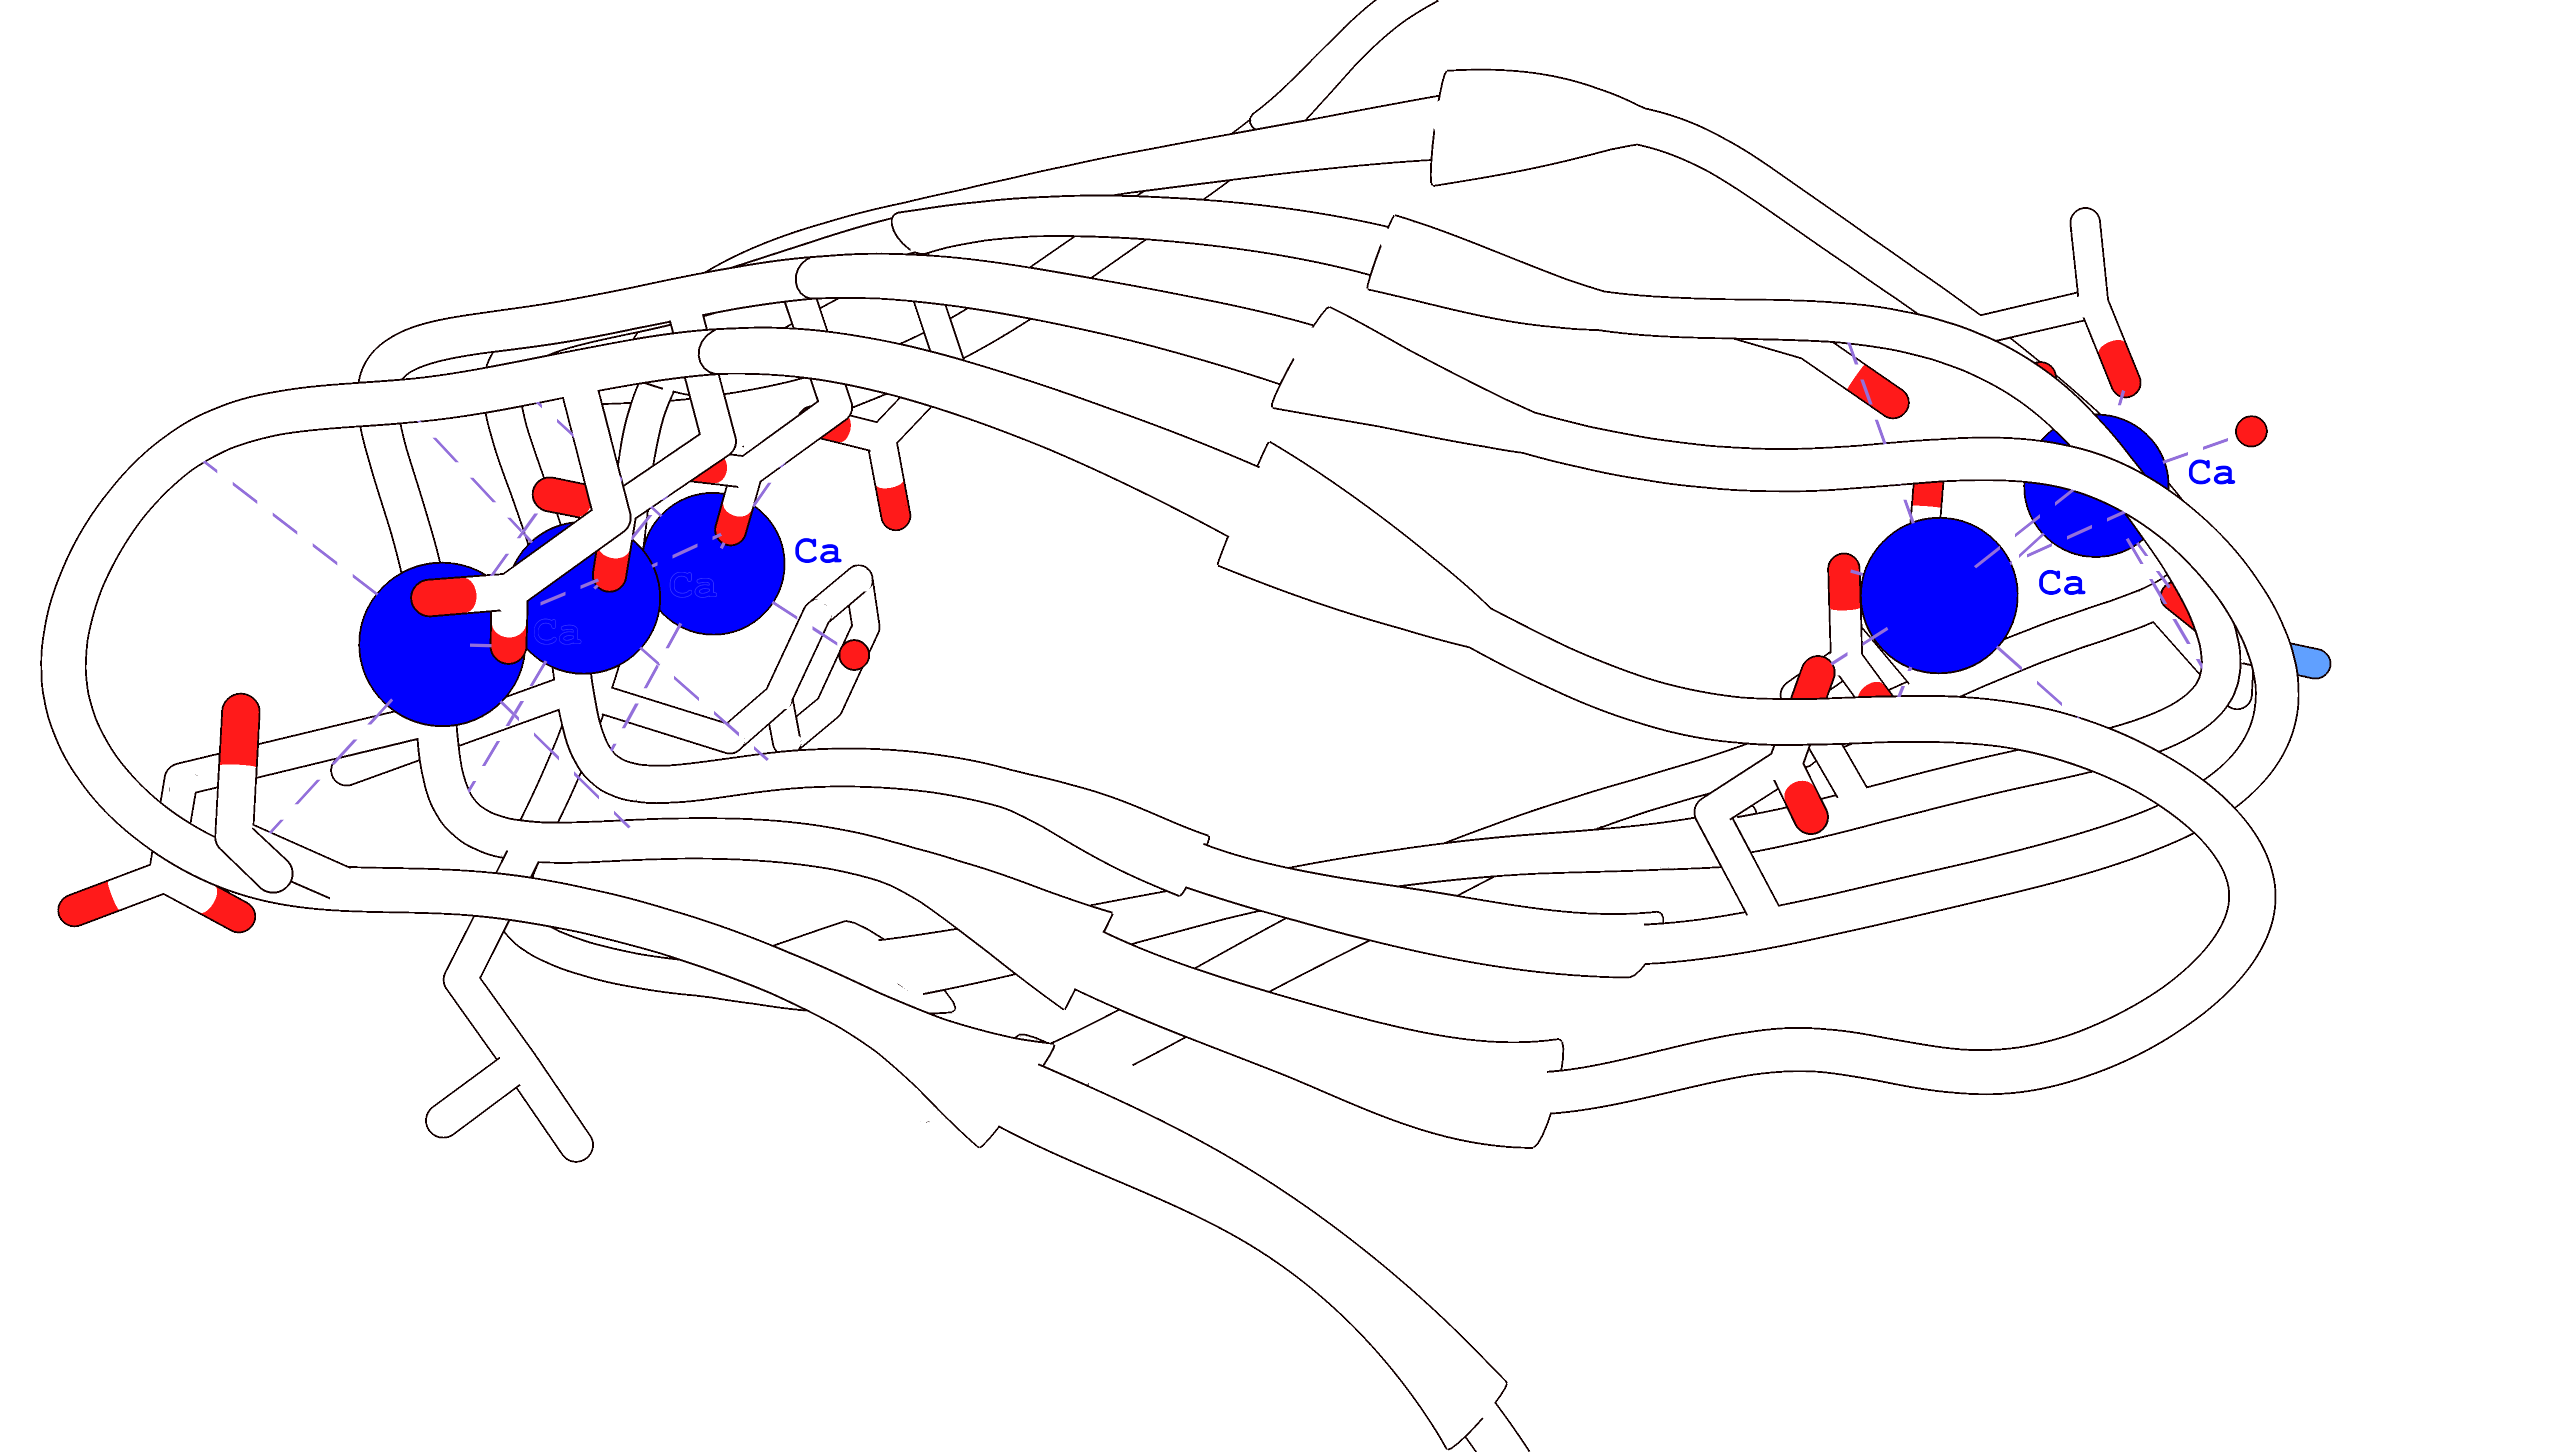
\includegraphics[width=0.7\textwidth]{intro/img/rtx-white.png}
    \end{center}

    \caption[The structure of \ac{rtx} motifs]{The structure of \ac{rtx} motifs. This view is down the barrel of an \ac{rtx} $\beta$-fold. The blue spheres are calcium ions coordinated by aspartate residues which are shown. This structure is of MIS38, an extracellular lipase from \ac{pseudomonas} (PDB:2Z8X). The structure here depicts five \ac{rtx} sites binding five \ce{Ca^2+} ions, RsaA from \caulobacter also has five \ac{rtx} motifs in close vicinity and my have a similar structure the presented structure above. See the sequence of RsaA on \cpageref{app:rsaseq}, \ac{rtx} sequences are bolded. Generated using the program \texttt{Chimera} (\fullcite{pettersen2004ucsf}).
    }
    \label{fig:intro-rtx}
  \end{figure}   

  \ac{rtx} motifs are always on the C-terminal side of \ac{t1ss} proteins, and are thus are in the leading part of the polypeptide to be loaded in to the secretion machinery and the first part to be secreted. It should be noted that bacterial intracellular \ce{Ca^2+} concentrations are extremely low, 90$\pm$10 \si{\nano\molar}, and extracellular \ce{Ca^2+} concentrations are high, 0.1--1 \millimolar\upcite[.]{gangola1987maintenance, norris1996calcium} It is thought that the roles of \ac{rtx} motifs in \ac{t1ss} proteins are to induce an intrinsically disorder C-terminus prior to secretion and to quickly  bind \ce{Ca^2+} and begin folding once the protein has started to emerge from the secretion machinery\upcite[.]{perez2010characterization, sotomayor2014disorder} The calcium-induced folding may help the thermodynamics of secretion, possibly assisting by pulling the protein out of the pore.  Despite the apparent importance of \ac{rtx} motifs in \ac{t1ss} proteins, they are not sufficient nor even necessary for secretion\upcite[]{felmlee1988alterations} but in at least the case of HlyA, in \ecoli, the \ac{rtx} repeats are required for proper folding, activity, and maximal secretion\upcite[.]{felmlee1988alterations} It has been thought that the folding of the \ac{rtx} motifs can act as an `intramolecular' chaperone; they fold quickly first then act as a nucleation point for the rest of the protein to fold on\upcite[.]{sotomayor2014disorder} 

  \section{Lipopolysaccharide} \label{sec:intro-lps}
  \subsection{General Structure of LPS}\label{sub:general-structre-lps} 
  \subsection{Extraction and Isolation of LPS} \label{sub:extr-isol-lps}
  \subsection{LPS and Immunology}\label{sub:lps-immuonolgy}
  \subsection{Other surface polysaccharides}\label{sub:other-surf-polysaccharides}
  \section{Porins} \label{sec:intro-porins}   
  \subsection{Functions of Porins}\label{sub:functions-porins}
  \subsection{Structure of Porins}\label{sub:structure-porins}


  